\chapter{Общие сведения о сетях}

\section{От централизованных систем к вычислительным сетям}

Концепция вычислительных сетей является логическим результатом эволюционного развития вычислительной техники и техники систем связи (передачи  данных).
Вычислительные системы прошли большой путь развития от централизованных систем обработки данных на базе отдельных компьютеров до распределенных систем обработки данных, частным случаем которых являются вычислительные сети.

\subsection{Централизованные системы обработки данных}

Первоначально компьютеры - большие, громоздкие и дорогие - представляли собой \textbf{\textit{централизованные системы обработки данных}} и предназначались для небольшого числа пользователей.
Проблема обеспечения доступа различных пользователей к такому компьютеру решалась либо в режиме пакетной обработки, либо в многотерминальном режиме.

При использовании \textbf{\textit{режима пакетной обработки}} пользователи подготавливали перфокарты, содержащие данные и команды программ и передавали их операторам, которые вводили эти карты в компьютер, а распечатанные результаты пользователи получали обычно только на следующий день.

В начале 60-х годов начали развиваться интерактивные \textbf{\textit{многотерминальные системы}} разделения времени, которые в какой-то степени позволили учесть интересы пользователей.
В таких системах компьютер отдавался в распоряжение сразу нескольким пользователям, каждый из которых получал в свое распоряжение терминал для ведения диалога с компьютером.
Так как время реакции вычислительной системы было достаточно мало, то пользователю была не слишком заметна параллельная работа компьютера с другими пользователями.

Вычислительные сети - частный случай распределенных систем обработки данных.

Компьютерные сети относятся к распределенным (или децентрализованным) вычислительным системам. Поскольку основным признаком распределенной вычислительной системы является наличие нескольких центров обработки данных, то наряду с компьютерными сетями к распределенным системам относят также мультипроцессорные компьютеры и многомашинные вычислительные комплексы.

\textbf{\textit{В мультипроцессорных компьютерах}} имеется несколько процессоров, каждый из которых может относительно независимо от остальных выполнять свою программу.
В мультипроцессоре существует общая для всех процессоров операционная система, которая оперативно распределяет вычислительную нагрузку между процессорами.
Взаимодействие между отдельными процессорами организуется наиболее простым способом - через общую оперативную память.

Сам по себе процессорный блок не является законченным компьютером и поэтому не может выполнять программы без остальных блоков мультипроцессорного компьютера - памяти и периферийных устройств.
Все периферийные устройства являются для всех процессоров мультипроцессорной системы общими.
Территориальную распределенность мультипроцессор не поддерживает - все его блоки располагаются в одном или нескольких близко расположенных конструктивах, как и у обычного компьютера.

Основное достоинство мультипроцессора - его высокая производительность, которая достигается за счет параллельной работы нескольких процессоров.
Так как взаимодействие процессоров через общую память происходит очень быстро, мультипроцессоры могут эффективно выполнять даже приложения с высокой степенью связи по данным.

Еще одним важным свойством мультипроцессорных систем является отказоустойчивость, то есть способность к продолжению работы при отказах некоторых элементов, например процессоров или блоков памяти при некотором уменьшении производительности.

\textbf{\textit{Многомашинная система}} - это вычислительный комплекс, включающий в себя несколько компьютеров (каждый из которых работает под управлением собственной операционной системы), а также программные и аппаратные средства связи компьютеров, которые обеспечивают работу всех компьютеров комплекса как единого целого.

Работа любой многомашинной системы определяется двумя главными компонентами: высокоскоростным механизмом связи процессоров и системным программным обеспечением, которое предоставляет пользователям и приложениям прозрачный доступ к ресурсам всех компьютеров, входящих в комплекс.
В состав средств связи входят программные модули, которые занимаются распределением вычислительной нагрузки, синхронизацией вычислений и реконфигурацией системы.
Если происходит отказ одного из компьютеров комплекса, его задачи могут быть автоматически переназначены и выполнены на другом компьютере.
Если в состав многомашинной системы входят несколько контроллеров внешних устройств, то в случае отказа одного из них, другие контроллеры автоматически подхватывают его работу.
Таким образом, достигается высокая отказоустойчивость комплекса в целом.

Помимо повышения отказоустойчивости, многомашинные системы позволяют достичь высокой производительности за счет организации параллельных вычислений.
Эффективность распараллеливания решаемых задач в многомашинных системах по сравнению с мультипроцессорными системами снижается, если параллельно выполняемые задачи тесно связаны между собой по данным.
Это объясняется тем, что обмен данными осуществляется через общие многовходовые периферийные устройства.
Территориальная распределенность в многомашинных комплексах не обеспечивается, так как расстояния между компьютерами определяются длиной связи между процессорным блоком и дисковой подсистемой.

Хронологически первыми появились глобальные вычислительные сети, так как первой назрела потребность в соединении компьютеров, находящихся на большом расстоянии друг от друга.

Началось все с решения более простой задачи - доступа к компьютеру с терминалов, удаленных от него на многие сотни, а то и тысячи километров.

Затем появились системы, в которых наряду с удаленными соединениями типа терминал-компьютер были реализованы и удаленные связи типа компьютер-компьютер.
Компьютеры получили возможность обмениваться данными в автоматическом режиме, что, собственно, и является базовым механизмом любой вычислительной сети.
Используя, этот механизм, в первых сетях были реализованы службы обмена файлами, синхронизации баз данных, электронной почты и другие, ставшие теперь традиционными сетевые службы.

Именно при построении глобальных сетей были впервые предложены и отработаны многие основные идеи и концепции современных вычислительных сетей.
Такие, например, как многоуровневое построение коммуникационных протоколов, технология коммутации пакетов, маршрутизация пакетов в составных сетях.

\subsection{Первые локальные сети}

В начале 70-х годов произошел технологический прорыв в области производства компьютерных компонентов - появились большие интегральные схемы.
Их сравнительно невысокая стоимость и высокие функциональные возможности привели к созданию мини-компьютеров, которые стали реальными конкурентами мэйнфреймов.
Даже небольшие подразделения предприятий получили возможность покупать для себя компьютеры, которые выполняли задачи управления технологическим оборудованием, складом и другие задачи уровня подразделения предприятия.
Таким образом, появилась концепция распределения компьютерных ресурсов по всему предприятию.
Однако при этом все компьютеры одной организации по-прежнему продолжали работать автономно.

Но шло время, потребности пользователей вычислительной техники росли, им стало недостаточно собственных компьютеров, им уже хотелось получить возможность обмена данными с другими близко расположенными компьютерами.
В ответ на эту потребность предприятия и организации стали соединять свои мини-компьютеры вместе и разрабатывать программное обеспечение, необходимое для их взаимодействия.
В результате появились первые локальные вычислительные сети.
Они во многом отличались от современных локальных сетей, в первую очередь - своими устройствами сопряжения.
На первых порах для соединения компьютеров друг с другом использовались самые разнообразные нестандартные устройства со своим способом представления данных на линиях связи, своими типами кабелей и т. п.
Эти устройства могли соединять только те типы компьютеров, для которых были разработаны.

\begin{figure}[!ht]
    \centering
    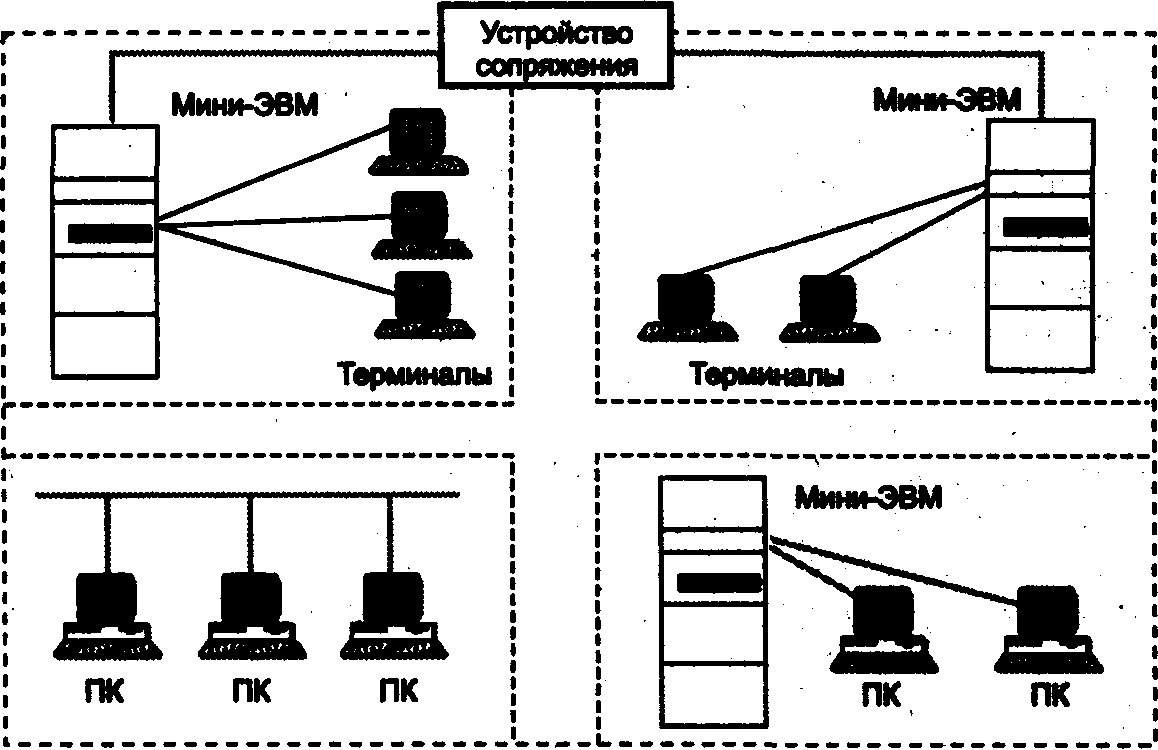
\includegraphics[width=0.7\textwidth]{connection-types.png}
    \caption{Различные типы связей в первых локальных сетях}
    \label{fig:connection-types}
\end{figure}

\subsection{Создание стандартных технологий локальных сетей}

В середине 80-х годов положение дел в локальных сетях стало кардинально меняться в связи с тем, что утвердились стандартные технологии объединения компьютеров в сеть - Ethernet, Arcnet, Token Ring.
Мощным стимулом для их развития послужили персональные компьютеры, которые при своей относительной дешевизне явились идеальными элементами для построения сетей - с одной стороны, они были достаточно мощными для работы сетевого программного обеспечения, а с другой - явно нуждались в объединении своей вычислительной мощности для решения сложных задач, а также разделения дорогих периферийных устройств и дисковых массивов.

Стандартные сетевые технологии превратили процесс построения локальной сети из искусства в рутинную работу.
Для создания сети достаточно было приобрести сетевые адаптеры соответствующего стандарта, например Ethernet, стандартный кабель, присоединить адаптеры к кабелю стандартными разъемами и установить на компьютер одну из сетевых операционных систем.
После этого, сеть начинала работать и присоединение каждого нового компьютера не вызывало никаких проблем - естественно, если на нем был установлен сетевой адаптер той же технологии.

\subsection{Основные программные и аппаратные компоненты сети}

Современная вычислительная сеть - это сложный комплекс взаимосвязанных и согласованно функционирующих программных и аппаратных компонентов.
Изучение сети в целом предполагает знание принципов работы ее отдельных элементов:
\begin{itemize}
    \item компьютеров;
    \item коммуникационного оборудования;
    \item операционных систем;
    \item сетевых приложений.
\end{itemize}

Весь комплекс программно-аппаратных средств сети может быть описан многослойной моделью.

В основе любой сети лежит аппаратный слой \textbf{\textit{стандартизованных компьютерных платформ}}.
В настоящее время в сетях широко и успешно применяются компьютеры различных классов - от персональных компьютеров до мэйнфреймов и суперЭВМ.
Набор компьютеров в сети должен соответствовать набору задач, решаемых сетью.

Второй слой - это \textbf{\textit{коммуникационное оборудование}}. В настоящее время кабельные системы, повторители, мосты, коммутаторы, маршрутизаторы и модульные концентраторы из вспомогательных компонентов сети превратились в основные наряду с компьютерами и системным программным обеспечением.

Третьим слоем, образующим программную платформу сети, являются \textbf{\textit{сетевые операционные системы (ОС)}}. От того, какие концепции управления локальными и распределенными ресурсами положены в основу сетевой ОС, зависит эффективность работы всей сети.

Самым верхним слоем сетевых средств являются различные \textbf{\textit{сетевые приложения}}, такие как сетевые базы данных, почтовые системы, средства архивирования данных, системы автоматизации коллективной работы и др.

\section{Основные проблемы построения сетей}
При создании вычислительных сетей их разработчикам пришлось решить много проблем.
Рассмотрим только наиболее важные из них, причем в той последовательности, в которой они естественно возникали в процессе развития и совершенствования сетевых технологий.

\subsection{Проблемы физической передачи данных по линиям связи}

Даже при рассмотрении простейшей сети, состоящей всего из двух машин, можно увидеть многие проблемы, присущие любой вычислительной сети, в том числе проблемы, связанные с физической передачей сигналов по линиям связи.

В вычислительной технике для представления данных используется двоичный код.
Внутри компьютера единицам и нулям данных соответствуют дискретные электрические сигналы.
Представление данных в виде электрических или оптических сигналов называется кодированием.
Существуют различные способы кодирования двоичных цифр 1 и 0, например, «потенциальный способ», при котором единице соответствует один уровень напряжения, а нулю - другой, или импульсный способ, когда для представления цифр используются импульсы различной (одной) полярности.

\begin{figure}[!ht]
    \centering
    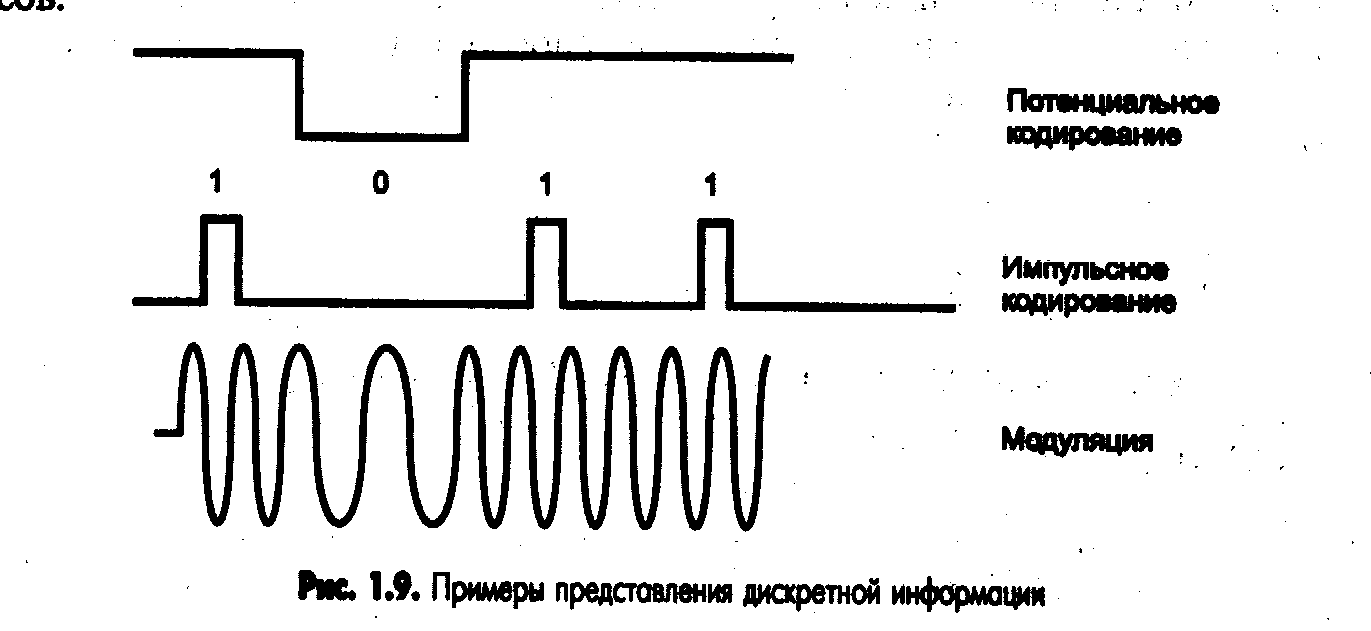
\includegraphics[width=0.5\textwidth]{discrete-information}
    \caption{Примеры представления дискретной информации}
    \label{fig:discrete-information}
\end{figure}

В вычислительных сетях применяют как \textbf{\textit{потенциальное, так и импульсное кодирование дискретных данных}}, а также специфический способ представления данных, который никогда не используется внутри компьютера, - \textbf{\textit{модуляцию}}.
Связано это с тем, что линии связи между компьютерами существенно отличаются по своим характеристикам от внутренних линий связи компьютера, прежде всего большей протяженностью, что приводит к увеличению паразитных параметров линии и, в конечном итоге, к уменьшению уровня и искажению сигнала.
При модуляции дискретная информация представляется синусоидальным сигналом той частоты, которую хорошо передает имеющаяся линия связи.

Потенциальное или импульсное кодирование применяется на каналах высокого качества, а модуляция на основе синусоидальных сигналов предпочтительнее в том случае, когда канал вносит сильные искажения в передаваемые сигналы.

На способ передачи сигналов влияет и количество проводов в линиях связи между компьютерами.
Для сокращения стоимости линий связи в сетях обычно стремятся к сокращению количества проводов и из-за этого используют не параллельную передачу всех бит одного байта или даже нескольких байт, как это делается внутри компьютера, а \textbf{\textit{последовательную, побитную передачу}}, требующую всего одной пары проводов.

Еще одной проблемой, которую нужно решать при передаче сигналов, является \textbf{\textit{проблема взаимной синхронизации передатчика одного компьютера с приемником другого}}.
При организации взаимодействия модулей внутри компьютера эта проблема решается очень просто, так как в этом случае все модули синхронизируются от общего тактового генератора.
Проблема синхронизации при связи компьютеров может решаться разными способами, как с помощью обмена специальными тактовыми синхроимпульсами по отдельной линии, так и с помощью периодической синхронизации заранее обусловленными кодами или импульсами характерной формы, отличающейся от формы импульсов данных.

\textbf{\textit{Несмотря на предпринимаемые меры}} - выбор соответствующей скорости обмена данными, линий связи с определенными характеристиками, способа синхронизации приемника и передатчика, - \textbf{\textit{существует вероятность искажения некоторых бит передаваемых данных}}.
Для повышения надежности передачи данных между компьютерами часто используется стандартный прием - подсчет контрольной суммы и передача ее по линиям связи после каждого байта или после некоторого блока байтов.
Часто в протокол обмена данными включается, как обязательный элемент сигнал-квитанция, который подтверждает правильность приема данных и посылается от получателя к отправителю.

Задачи надежного обмена двоичными сигналами, представленными соответствующими электромагнитными сигналами, в вычислительных сетях решает определенный класс оборудования.
В локальных сетях это \emph{сетевые адаптеры}, в глобальных сетях - аппаратура передачи данных, к которой относятся, например, устройства, выполняющие модуляцию и демодуляцию дискретных сигналов, - \emph{модемы}.
Это оборудование кодирует и декодирует каждый информационный бит, синхронизирует передачу электромагнитных сигналов по линиям связи, проверяет правильность передачи по контрольной сумме и может выполнять некоторые другие операции.

\subsection{Проблемы объединения нескольких компьютеров}

До сих пор мы рассматривали вырожденную сеть, состоящую всего из двух машин.
При объединении в сеть большего числа компьютеров возникает целый комплекс новых проблем.

\subsection{Топология физических связей}

В первую очередь необходимо выбрать способ организации физических связей, то есть топологию.
Под топологией вычислительной сети понимается конфигурация графа, вершинам которого соответствуют компьютеры сети (иногда и другое оборудование, например концентраторы), а ребрам - физические связи между ними.
Компьютеры, подключенные к сети, часто называют станциями или узлами сети.

Заметим, что конфигурация физических связей определяется электрическими соединениями компьютеров между собой и может отличаться от конфигурации логических связей между узлами сети.
Логические связи представляют собой маршруты передачи данных между узлами сети и образуются путем соответствующей настройки коммуникационного оборудования.

Выбор топологии электрических связей существенно влияет на многие характеристики сети.
Например, наличие резервных связей повышает надежность сети и делает возможным балансирование загрузки отдельных каналов.
Простота присоединения новых узлов, свойственная некоторым топологиям, делает сеть легко расширяемой.
Экономические соображения часто приводят к выбору топологий, для которых характерна минимальная суммарная длина линий связи.

Рассмотрим некоторые, наиболее часто встречающиеся топологии:
\begin{itemize}
    \item полносвязная топология;
    \item ячеистая топология;
    \item общая шина;
    \item звезда;
    \item кольцо.
\end{itemize}

\begin{figure}[!ht]
    \centering
    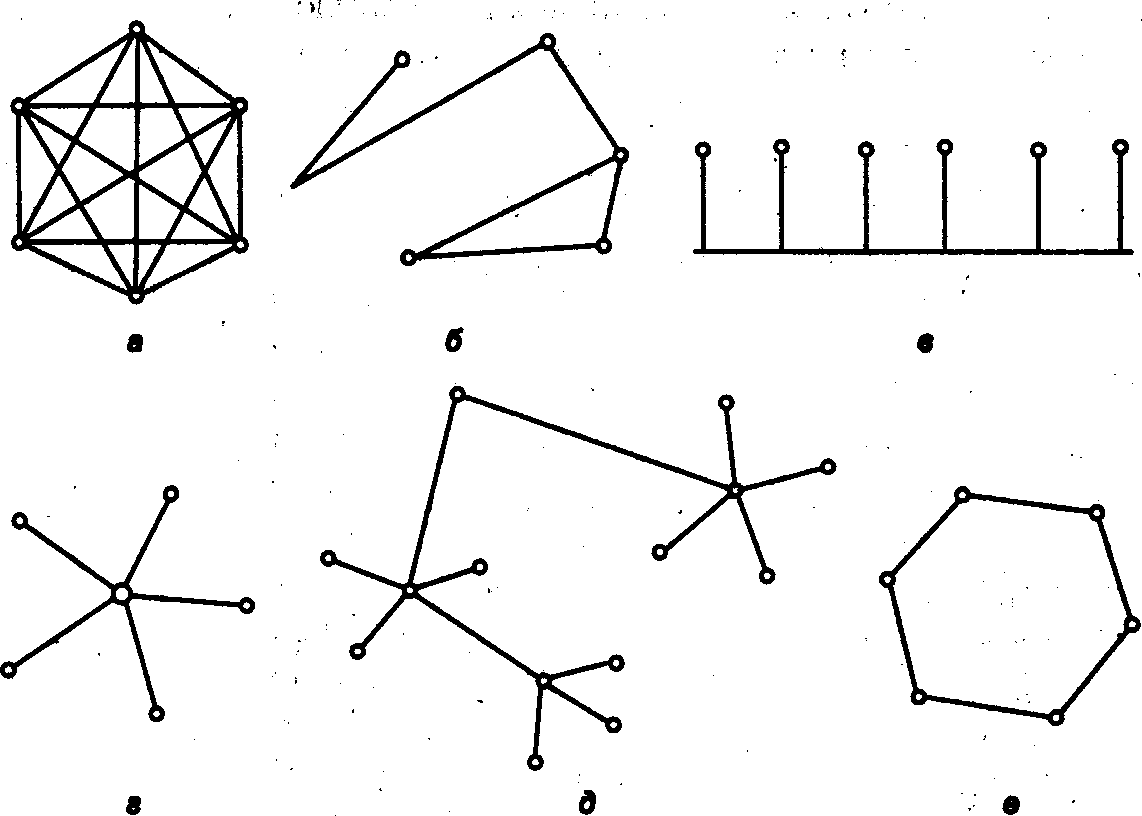
\includegraphics[width=0.5\textwidth]{topologies}
    \caption{Распространённые топологии}
    \label{fig:topologies}
\end{figure}

\textbf{\textit{Полносвязная топология}} соответствует сети, в которой каждый компьютер сети связан со всеми остальными.
Несмотря на логическую простоту, этот вариант оказывается громоздким и неэффективным.
Действительно, каждый компьютер в сети должен иметь большое количество коммуникационных портов, достаточное для связи с каждым из остальных компьютеров сети.
Для каждой пары компьютеров должна быть выделена отдельная электрическая линия связи.
Полносвязные топологии применяются редко и чаще всего используются в многомашинных комплексах.

\textbf{\textit{Ячеистая топология (mesh)}} получается из полносвязной путем удаления некоторых возможных связей.
В сети с ячеистой топологией непосредственно связываются только те компьютеры, между которыми происходит интенсивный обмен данными, а для обмена данными между компьютерами, не соединенными прямыми связями, используются транзитные передачи через промежуточные узлы.
Ячеистая топология допускает соединение большого количества компьютеров и характерна, как правило, для глобальных сетей.

\textbf{\textit{Общая шина}} является очень распространенной (а до недавнего времени самой распространенной) топологией для локальных сетей.
В этом случае компьютеры подключаются к одному коаксиальному кабелю по схеме «монтажного ИЛИ».
Передаваемая информация может распространяться в обе стороны.
Применение общей шины снижает стоимость проводки, унифицирует подключение различных модулей, обеспечивает возможность почти мгновенного широковещательного обращения ко всем станциям сети.
Таким образом, основными преимуществами такой схемы являются дешевизна и простота разводки кабеля по помещениям.
Самый серьезный недостаток общей шины заключается в ее низкой надежности: любой дефект кабеля или какого-нибудь из многочисленных разъемов полностью парализует всю сеть.
К сожалению, дефект коаксиального разъема редкостью не является.
Другим недостатком общей шины является ее невысокая производительность, так как при таком способе подключения в каждый момент времени только один компьютер может передавать данные в сеть.
Поэтому пропускная способность канала связи всегда делится здесь между всеми узлами сети.

\textbf{\textit{Топология звезда}} предполагает, что каждый компьютер подключается отдельным кабелем к общему устройству, называемому хостом или концентратором, который находится в центре сети.
В функции концентратора входит направление передаваемой компьютером информации одному или всем остальным компьютерам сети.
Главное преимущество этой топологии перед общей шиной - существенно большая надежность.
Любые неприятности с кабелем касаются лишь того компьютера, к которому этот кабель присоединен, и только неисправность концентратора может вывести из строя всю сеть.
Кроме того, концентратор может играть роль интеллектуального фильтра информации, поступающей от узлов в сеть, и при необходимости блокировать запрещенные администратором передачи.

К недостаткам топологии типа звезда относится более высокая стоимость сетевого оборудования из-за необходимости приобретения концентратора.
Кроме того, возможности по наращиванию количества узлов в сети ограничиваются количеством портов концентратора.
Иногда имеет смысл строить сеть с использованием нескольких концентраторов, иерархически соединенных между собой связями типа звезда.
В настоящее время иерархическая звезда является самым распространенным типом топологии связей как в локальных, так и глобальных сетях.

В сетях с \textbf{\textit{кольцевой конфигурацией}} данные передаются по кольцу от одного компьютера к другому, как правило, в одном направлении.
Если компьютер распознает данные как «свои», то он копирует их себе во внутренний буфер.
В сети с кольцевой топологией необходимо принимать специальные меры, чтобы в случае выхода из строя или отключения какой-либо станции не прервался канал связи между остальными станциями.
Кольцо представляет собой очень удобную конфигурацию для организации обратной связи - данные, сделав полный оборот, возвращаются к узлу-источнику.
Поэтому этот узел может контролировать процесс доставки данных адресату.
Часто это свойство кольца используется для тестирования связности сети и поиска узла, работающего некорректно.
Для этого в сеть посылаются специальные тестовые сообщения.

В то время как небольшие сети, как правило, имеют типовую топологию - звезда, кольцо или общая шина, для крупных сетей характерно наличие произвольных связей между компьютерами.
В таких сетях можно выделить отдельные произвольно связанные фрагменты (подсети), имеющие типовую топологию, поэтому их называют сетями со смешанной топологией.

\begin{figure}[!ht]
    \centering
    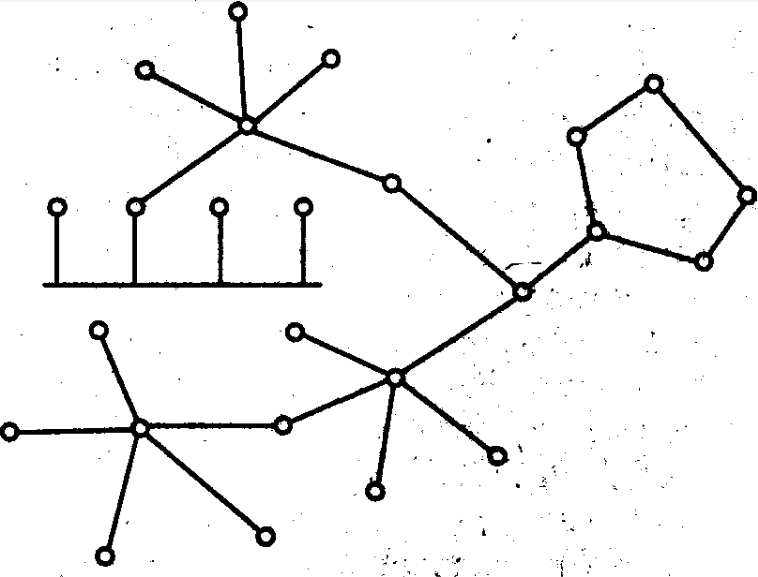
\includegraphics[width=0.5\textwidth]{mixed-topology}
    \caption{Смешанная топология}
    \label{fig:mixed-topology}
\end{figure}

\subsection{Организация совместного использования линий связи}

В вычислительных сетях используют как \textbf{\textit{индивидуальные линии связи между компьютерами}}, так и \textbf{\textit{разделяемые (shared)}}, когда одна линия связи попеременно используется несколькими компьютерами.
В случае применения разделяемых линий связи (часто используется также термин разделяемая среда передачи данных - shared media) возникает комплекс проблем, связанных с их совместным использованием.
Это как чисто электрические проблемы обеспечения нужного качества сигналов при подключении к одному и тому же проводу нескольких приемников и передатчиков, так и логические проблемы разделения во времени доступа к этим линиям.

Несмотря на все эти сложности, в локальных сетях разделяемые линии связи используются очень часто.
Этот подход, в частности, реализован в широко распространенных классических технологиях Ethernet и Token Ring.
Однако в последние годы наметилась тенденция отказа от разделяемых сред передачи данных и в локальных сетях.
Это связано с тем, что за достигаемое таким образом удешевление сети приходится расплачиваться производительностью.

\subsection{Адресация компьютеров}

Еще одной новой проблемой, которую нужно учитывать при объединении трех и более компьютеров, является проблема их адресации.
К адресу узла сети и схеме, его назначения можно предъявить несколько требований.
\begin{itemize}
    \item Адрес должен уникально идентифицировать компьютер в сети любого масштаба.
    \item Схема назначения адресов должна сводить к минимуму ручной труд администратора и вероятность дублирования адресов.
    \item Адрес должен иметь иерархическую структуру, удобную для построения больших сетей.
        Эту проблему хорошо иллюстрируют международные почтовые адреса, которые позволяют почтовой службе, организующей доставку писем между странами, пользоваться только названием страны адресата и не считывать название его города, а тем более улицы.
    \item Адрес должен быть удобен для пользователей сети, а это значит, что он должен иметь символьное представление, например, Server или www.dsCo.com.
    \item Адрес должен иметь по возможности компактное представление, чтобы не перегружать память коммуникационной аппаратуры - сетевых адаптеров,  маршрутизаторов и т. п.
\end{itemize}

Нетрудно заметить, что эти требования противоречивы - например, адрес, имеющий иерархическую структуру, скорее всего, будет менее компактным, чем неиерархический (такой адрес часто называют «плоским», то есть не имеющим структуры).
Символьный же адрес, скорее всего, потребует больше памяти, чем адрес-число.

Так как все перечисленные требования трудно совместить в рамках какой-либо одной схемы адресации, то на практике обычно используется сразу несколько схем, так что компьютер одновременно имеет несколько адресов-имен.
Каждый адрес используется в той ситуации, когда соответствующий вид адресации наиболее удобен.
А чтобы не возникало путаницы, и компьютер всегда однозначно определялся своим адресом, используются специальные вспомогательные протоколы, которые по адресу одного типа могут определить адреса других типов.

Наибольшее распространение получили три схемы адресации узлов.
\begin{itemize}
    \item Аппаратные (hardware) адреса.
        Эти адреса предназначены для сети небольшого или среднего размера, поэтому они не имеют иерархической структуры, Типичным представителем адреса такого типа является адрес сетевого адаптера локальной сети.
        Такой адрес обычно используется только аппаратурой, поэтому его стараются сделать по возможности компактным и записывают в виде двоичного или шестнадцатеричного значения, например 0081005е24а8.
        При задании аппаратных адресов обычно не требуется выполнение ручной работы, так как они либо встраиваются в аппаратуру компанией-изготовителем, либо генерируются автоматически при каждом новом запуске оборудования, причем уникальность адреса в пределах сети обеспечивает оборудование.
        Помимо отсутствия иерархии, использование аппаратных адресов связано еще с одним недостатком - при замене аппаратуры, например, сетевого адаптера, изменяется и адрес компьютера.
        Более того, при установке нескольких сетевых адаптеров у компьютера появляется несколько адресов, что не очень удобно для пользователей сети.
    \item Символьные адреса или имена.
        Эти адреса предназначены для запоминания людьми и поэтому обычно несут смысловую нагрузку.
        Символьные адреса легко использовать как в небольших, так и крупных сетях.
        Для работы в больших сетях символьное имя может иметь сложную иерархическую структуру, например ftp-archl.ucl.ac.uk.
        Этот адрес говорит о том, что данный компьютер поддерживает ftp-архив в сети одного из колледжей Лондонского университета (University College London - ucl) и эта сеть относится к академической ветви (ac) Internet Великобритании (United Kingdom - uk).
        При работе в пределах сети Лондонского университета такое длинное символьное имя явно избыточно и вместо него удобно пользоваться кратким символьным именем, на роль которого хорошо подходит самая младшая составляющего полного имени, то есть имя ftp-archl.
    \item Числовые составные адреса.
        Символьные имена удобны для людей, но из-за переменного формата и потенциально большой длины их передача по сети не очень экономична.
        Поэтому во многих случаях для работы в больших сетях в качестве адресов узлов используют числовые составные адреса фиксированного и компактного форматов.
\end{itemize}

Типичным представителями адресов этого типа являются IP- и IPX-адреса.
В них поддерживается двухуровневая иерархия, адрес делится на старшую часть - номер сети и младшую - номер узла.
Такое деление позволяет передавать сообщения между сетями только на основании номера сети, а номер узла используется только после доставки сообщения в нужную сеть; точно так же, как название улицы используется почтальоном только после того, как письмо доставлено в нужный город.

В последнее время, чтобы сделать маршрутизацию в крупных сетях более эффективной, предлагаются более сложные варианты числовой адресации, в соответствии с которыми адрес имеет три и более составляющих.
Такой подход, в частности, реализован в новой версии протокола IPv6, предназначенного для работы в сети Internet.

\section{Структуризация как средство построения больших сетей}

В сетях с небольшим (10-30) количеством компьютеров чаще всего используется одна из типовых топологий - общая шина, кольцо или звезда.
Все перечисленные топологии обладают свойством однородности, то есть все компьютеры в такой сети имеют одинаковые права в отношении доступа к другим компьютерам (за исключением центрального компьютера при соединении звезда).
Такая однородность структуры делает простой процедуру наращивания числа компьютеров, облегчает обслуживание и эксплуатацию сети.

Однако при построении больших сетей, однородная структура связей превращается из преимущества в недостаток.
В таких сетях использование типовых структур порождает различные ограничения, важнейшими из которых являются:
\begin{itemize}
    \item ограничения на длину связей между узлами;
    \item ограничения на количество узлов в сети;
    \item ограничения на интенсивность трафика, порождаемого узлами сети.
\end{itemize}

Например, технология Ethernet на тонком коаксиальном кабеле позволяет использовать кабель длиной не более 185 метров, к которому можно подключить не более 30 компьютеров.
Однако, если компьютеры интенсивно обмениваются информацией между собой, иногда приходится снижать число подключенных к кабелю компьютеров до 20, а то и до 10, чтобы каждому компьютеру доставалась приемлемая доля общей пропускной способности сети.

Для снятия этих ограничений используются специальные методы структуризации сети и специальное структурообразующее коммуникационное оборудование - повторители, концентраторы, мосты, коммутаторы, маршрутизаторы.

\subsection{Физическая структуризация}
Простейшее из коммуникационных устройств – \textbf{\textit{повторитель (repeator)}} - используется для физического соединения различных сегментов кабеля локальной сети с целью увеличения общей длины сети.
Повторитель передает сигналы, приходящие из одного сегмента сети, в другие ее сегменты и позволяет преодолеть ограничения на длину линий связи за счет улучшения качества передаваемого сигнала - восстановления его мощности и амплитуды, улучшения фронтов и т.п.

Повторитель, который имеет несколько портов и соединяет несколько физических сегментов, часто называют \textbf{\textit{концентратором (concentrator)}} или \textbf{\textit{хабом (hub)}}.
Эти названия (hub - основа, центр деятельности) отражают тот факт, что в данном устройстве сосредоточиваются все связи между сегментами сети.

Концентраторы характерны практически для всех базовых технологий локальных сетей - Ethernet, ArcNet, Token Ring, FDDI, Fast Ethernet, Gigabit Ethernet, l00VG-AnyLAN.

Нужно подчеркнуть, что в работе концентраторов любых технологий много общего - они повторяют сигналы, пришедшие с одного из своих портов, на других своих портах.
Разница состоит в том, на каких именно портах повторяются входные сигналы.
Так, концентратор Ethernet повторяет входные сигналы на всех своих портах, кроме того, с которого сигналы поступают.
А концентратор Token Ring повторяет входные сигналы, поступающие с некоторого порта, только на одном порту - на том, к которому подключен следующий в кольце компьютер.

\textbf{\underline{ВНИМАНИЕ}} Концентратор всегда изменяет физическую топологию сети, но при этот оставляет без изменения ее логическую топологию.

\subsection{Логическая структуризация сети}

Физическая структуризация сети полезна во многих отношениях, однако, в ряде случаев невозможно обойтись без логической структуризации сети.
Наиболее важной проблемой, не решаемой путем физической структуризации, остается проблема перераспределения передаваемого трафика между различными физическими сегментами сети.

Решение проблемы состоит в отказе от идеи единой однородной разделяемой среды.
Например, в рассмотренном выше примере желательно было бы сделать так, чтобы кадры, которые передают компьютеры отдела 1, выходили бы за пределы этой части сети только в том случае, если эти кадры направлены какому-либо компьютеру из других отделов.
С другой стороны, в сеть каждого из отделов должны попадать только те кадры, которые адресованы узлам этой сети.
При такой организации работы сети ее производительность существенно повысится, так как компьютеры одного отдела не будут простаивать в то время, когда обмениваются данными компьютеры других отделов.

В предложенном решении мы отказались от идеи общей разделяемой среды в пределах всей сети, хотя и оставили ее в пределах каждого отдела.
Пропускная способность линий связи между отделами не должна совпадать с пропускной способностью среды внутри отделов.
Величина пропускной способности линий связи и коммуникационного оборудования, соединяющего отделы, определяется интенсивностью трафика между ними.

Распространение трафика, предназначенного для компьютера некоторого сегмента сети, только в пределах этого сегмента, называется \emph{локализацией трафика}.
\emph{Логическая структуризация сети} - это процесс разбиения сети на сегменты с локализованным трафиком.

Для логической структуризации сети используются такие коммуникационные устройства, как:
\begin{itemize}
    \item мосты;
    \item коммутаторы;
    \item маршрутизаторы;
    \item шлюзы.
\end{itemize}

\textbf{\textit{Мост (bridge)}} делит разделяемую среду передачи сети на части (часто называемые логическими сегментами), передавая информацию из одного сегмента в другой только в том случае, если адрес компьютера назначения принадлежит другой подсети.
Тем самым мост изолирует трафик одной подсети от трафика другой, повышая общую производительность передачи данных в сети.
Локализацией трафика также можно уменьшить возможность несанкционированного доступа к данным, так как кадры не выходят за пределы своего сегмента и их сложнее перехватить извне.

\begin{figure}[!ht]
    \centering
    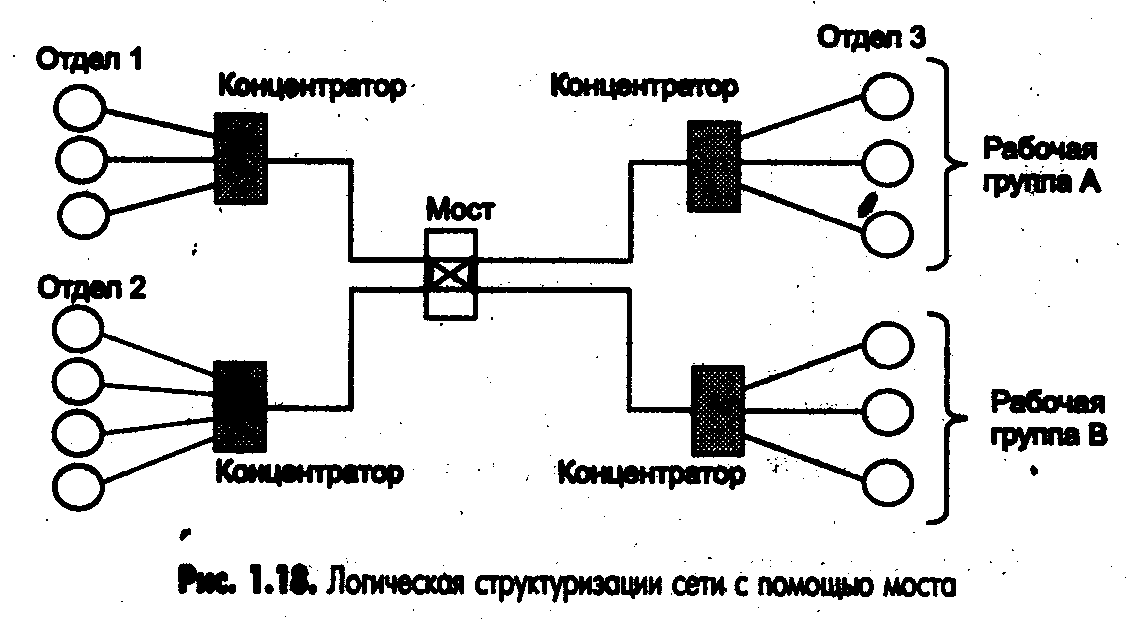
\includegraphics[width=0.5\textwidth]{logic-structure-with-bridge}
    \caption{Логическая структуризация сети с помощью маршрутизаторов}
    \label{fig:logic-structure-with-bridge}
\end{figure}

На рисунке показана сеть, которая была получена из рассмотренной нами ранее сети с центральным концентратором путем его замены на мост.
Сети 1-го и 2-го отделов состоят из отдельных логических сегментов, а сеть отдела 3 - из двух логических сегментов.
Каждый логический сегмент построен на базе концентратора и имеет простейшую физическую структуру, образованную отрезками кабеля, связывающими компьютеры с портами концентратора.

Мосты используют для локализации трафика аппаратные адреса компьютеров, которые не содержат никакой информации о принадлежности компьютера к сегменту.
Поэтому мост достаточно упрощенно представляет деление сети на сегменты - он запоминает, через какой порт на него поступил кадр данных от каждого компьютера сети, и в дальнейшем передает кадр, предназначенные для этого компьютера, на этот порт.
Точной топологии связей между логическими сегментами мост не знает.
Из-за этого применение мостов приводит к значительным ограничениям на конфигурацию связей сети - сегменты должны быть соединены таким образом, чтобы в сети не образовывались замкнутые контуры.

\textbf{\textit{Коммутатор (switch, switching hub)}} no принципу обработки кадров ничем не отличается от моста.
Основное его отличие от моста состоит в том, что он является своего рода коммуникационным мультипроцессором, так как каждый его порт оснащен специализированным процессором, который обрабатывает кадры по алгоритму моста независимо от процессоров других портов.
За счет этого общая производительность коммутатора обычно намного выше производительности традиционного моста, имеющего один процессорный блок.
Можно сказать, что коммутаторы - это мосты нового поколения, которые обрабатывают кадры в параллельном режиме.

Ограничения, связанные с применением мостов и коммутаторов - по топологии связей, а также ряд других, - привели к тому, что в ряду коммуникационных устройств появился еще один тип оборудования - \textbf{\textit{маршрутизатор (router)}}.
Маршрутизаторы более надежно и более эффективно, чем мосты, изолируют трафик отдельных частей сети друг от друга.
Маршрутизаторы образуют логические сегменты посредством явной адресации, поскольку используют не плоские аппаратные, а числовые составные (иерархические) адреса.
В этих адресах имеется поле номера сети, так что все компьютеры, у которых значение этого поля одинаково, принадлежат к одному сегменту, называемому в данном случае подсетью (subnet).

Кроме локализации трафика маршрутизаторы выполняют еще много других полезных функций.
Так, маршрутизаторы могут работать в сети с замкнутыми контурами, при этом они осуществляют выбор наиболее рационального маршрута из нескольких возможных.
Сеть, представленная на рисунке, отличается от своей предшественницы, построенной на основе моста, тем, что между подсетями отделов 1 и 2 проложена дополнительная связь, которая может использоваться как для повышения производительности сети, так и для повышения ее надежности.

\begin{figure}[!ht]
    \centering
    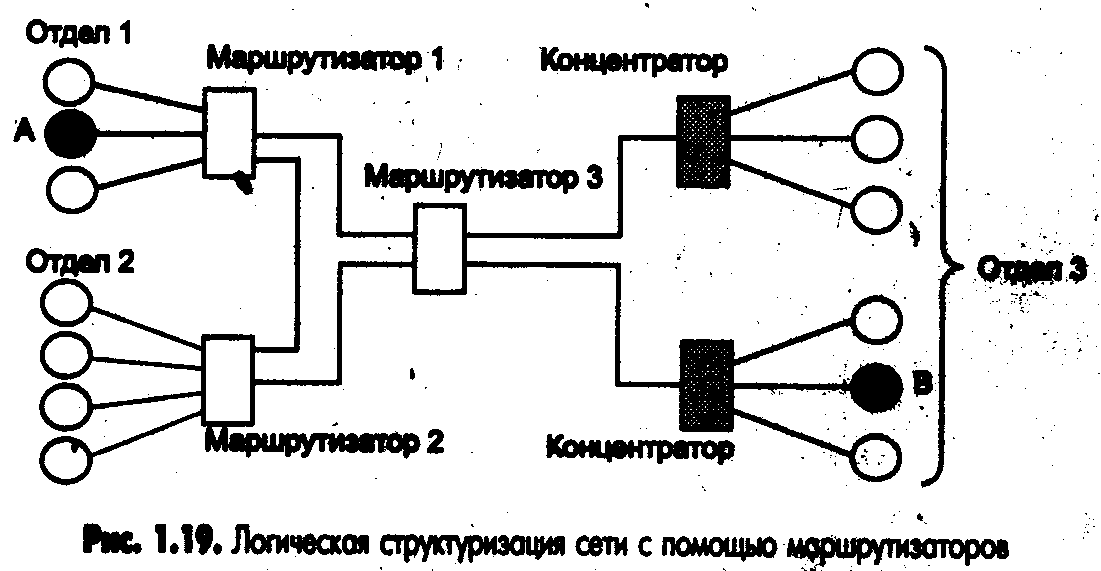
\includegraphics[width=0.5\textwidth]{logic-structure-with-router}
    \caption{Логическая структуризация сети с помощью маршрутизаторов}
    \label{fig:logic-structure-with-router}
\end{figure}

Другой очень важной функцией маршрутизаторов является их способность связывать в единую сеть подсети, построенные с использованием разных сетевых технологий, например Ethernet и Х.25.

Кроме перечисленных ранее устройств отдельные части сети может соединять \textbf{\textit{шлюз (gateway)}}.
Обычно основной причиной, по которой в сети используют шлюз, является необходимость объединить сети с разными типами системного и прикладного программного обеспечения, а не желание локализовать трафик.
Тем не менее, шлюз обеспечивает и локализацию трафика в качестве некоторого побочного эффекта.

Крупные сети практически никогда не строятся без логической структуризации.
Для отдельных сегментов и подсетей характерны типовые однородные топологии базовых технологий, и для их объединения всегда используется оборудование, обеспечивающее локализацию трафика, - мосты, коммутаторы, маршрутизаторы и шлюзы.
